\documentclass{article}
\usepackage{tikz, comment}
\usepackage{pifont}
\usepackage{fontspec}
\usetikzlibrary{arrows, decorations.markings, decorations.pathreplacing}
\begin{comment}
:Title: Not defined yet
:Slug: No name yet

Description Here.........
\end{comment}
\begin{document}\centering

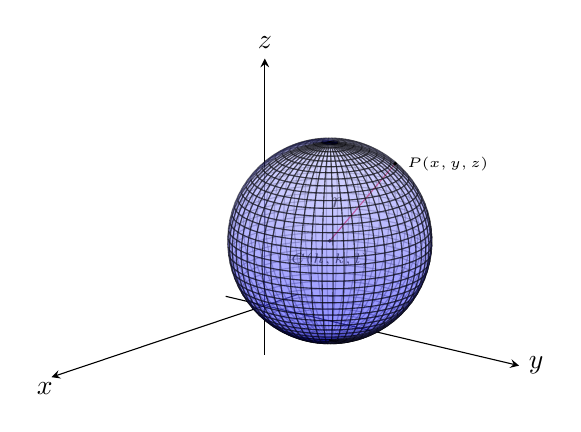
\begin{tikzpicture}[font=\footnotesize]

\pgfplotsset{
    colormap/outside/.style={
        colormap=
            {outside}{
            rgb255(0cm)=(110,110,255);
            rgb255(1cm)=(20,20,255);
            }
    },
    colormap/outside,
    colormap/inside/.style={
        colormap={inside}{
            rgb255(0cm)=(20,20,255);
            rgb255(1cm)=(220,220,255);
        }
    },
    colormap/inside
}

\pgfplotsset{compat=1.8}
\begin{axis}
[axis lines = center, view={130}{20}, scale=1, ticks=none, opacity=1, %height=4cm,width=6cm,
axis background, xlabel = {\normalsize $x$}, ylabel ={\normalsize $y$}, zlabel ={\normalsize $z$}, domain =-2:2, y domain =-2:2,
xmin =-0.5,
xmax = 3.25,
ymin =-0.5,
ymax = 3.25,
zmin =-0.5, 
zmax =2.5,
samples =10, samples y =40, z buffer = auto, 
every axis x label/.style={
    at={(ticklabel* cs:1)},
    anchor= east, xshift = 4, yshift=-4
},
every axis y label/.style={
    at={(ticklabel* cs:1)},
    anchor= west, xshift=0, yshift = 0
},
every axis z label/.style={
    at={(ticklabel* cs:1)},
    anchor= south
}]

    \addplot3 [
      surf, 
      domain=0:180,
      samples=40,
      y domain=135:315,
      samples y=30,
      line join=round, 
      mesh/interior colormap name=inside,
      colormap/outside,
      shader=faceted,
      variable=\t,
      point meta={cos(t)},
      faceted color=black, opacity=0.2
    ]
           ({0.5+1*sin(t)*cos(y)}, {1.25+1*sin(t)*sin(y)}, {1+1*cos(t)}); 

\addplot3[purple] coordinates
        {(0.5,1.25,1) ({0.5+1*sin(40)*cos(135)}, {1.25+1*sin(40)*sin(135)}, {1+1*cos(40)})};

\node[label={-90:{\tiny$C(h,k,l)$}},circle, black, fill, inner sep= 0.5pt] at (axis cs:0.5,1.25,1) {}; 
\node[label={180:{$r$}}] at (axis cs:0.27274, 1.47726, 1.38302) {};


    \addplot3 [
      surf, 
      domain=0:180,
      samples=40,
      y domain=-45:135,
      samples y=30,
      line join=round, 
      mesh/interior colormap name=inside,
      colormap/outside,
      shader=faceted,
      variable=\t,
      point meta={cos(t)},
      faceted color=black, opacity=0.5
    ]
           ({0.5+1*sin(t)*cos(y)}, {1.25+1*sin(t)*sin(y)}, {1+1*cos(t)});                       
         
\node[label={ 0:{\tiny$P(x,y,z)$}},circle, black, fill, inner sep= 0.5pt] at (axis cs:0.0454805, 1.70452, 1.76604) {}; 

\end{axis}

\end{tikzpicture}
\end{document}